\documentclass[a4paper,11pt]{article}

\usepackage[english]{babel}
\usepackage[utf8x]{inputenc}
\usepackage{amsmath}
\usepackage{graphicx}
\usepackage[margin=0.5in]{geometry}


\begin{document}

{\Huge Convergent Cross Mapping (CCM) Notes}

\hfill\rule{150mm}{.1pt}

\hfill{\small \today}

\section{Basic Idea}
Convergent cross mapping (CCM) is introduced in {\em Detecting Causality in
Complex Ecosystems}\footnote{http://www.uvm.edu/$\sim$cdanfort/csc-reading-group/sugihara-causality-science-2012.pdf} by Sugihara {\em et. al.}.  The supplementary text for that paper is very helpful\footnote{http://www.sciencemag.org/content/suppl/2012/09/19/science.1227079.DC1/Sugihara.SM.pdf}, although care should be taken when comparing the figure numbers between the text documents (the figure numbers in the supplementary text seem to be off by one).

CCM is a technique used to identify ``causality'' between time series and is intended to be useful in situations where the only other statistical ``causality'' measure, Granger causality, is known to be invalid (i.e.\ in dynamic systems that are ``nonseperable'').  The authors state that CCM is a ``necessary condition for causation'', but it may be best to avoid all discussion of causality in this work.  It is well known (refs would be nice) that Granger causality is unrelated to causality as it is typically understood in physics.  As such, rather than consider the necessity and sufficiency of CCM for causation, we will use the term ``directed correlation''. 

CCM is very similar to simplex projection, which was introduced by Sugihara and May in {\em Nonlinear forecasting as a way of distinguishing chaos from measurement error}\footnote{http://simplex.ucsd.edu/SugiMay-Chaos.pdf} and {\em Determining error from chaos in ecological time series}\footnote{http://simplex.ucsd.edu/SugiGrenMay-Chaos.pdf}.  A concise overview of simplex projection can be found online\footnote{http://simplex.ucsd.edu/}.  Simplex projection uses the points with the most similar histories to the point at $t$ to predict the point at $t+1$.  Similarly, CCM uses points with the most similar histories to a point $X(t)$ (in a time series $X$) to estimate the point $Y(t)$ (in a time series $Y$).

\section{Algorithm}
The algorithm (as it has been implemented here in Matlab) consists of five steps:
\begin{enumerate}
\item Create the shadow manifold for $X$, called $M_X$
\item Find the nearest neighbours to $X(t)$ in $M_X$
\item Use the nearest neighbours to create weights
\item Use the weights to estimate $Y(t)$, called $Y(t)|M_X$
\item Find the correlation between $Y(t)$ and $Y(t)|M_X$ (this correlation is what is reported as the ``directed correlation'')
\end{enumerate}
The steps vary in complexity and are explained in more detail below.

\subsection{Create $M_X$}
Given an embedding dimension $E$, the shadow manifold of $X$, called $M_X$, is created by associating an $E$-dimensional vector to each point $X(t)$ that is constructed as $\vec{X}(t)=(X(t),X(t-\tau),X(t-2\tau),\ldots,X(t-(E-1)\tau)$.  The first such vector is created at $t=1+(E-1)\tau\equiv t_s$ and the last is at $t=L\equiv t_l$ where $L$ is the time series length (or ``library length'').  The shadow manifold of $X$ is the collection of all such vectors, i.e.\ $M_X=\{\vec{X}(t) | t\in[t_s,t_l]\}$.  The time step $\tau$ is not discussed much in any of the Sugihara papers, and it appears to always be assumed that $\tau=1$.  We will follow that assumption throughout these notes unless specifically stated otherwise.    

\subsection{Find Nearest Neighbours}
The minimum number of points required for a bounding simplex in an $E$-dimensional space is $E+1$ (find a non-Sugihara reference for this statement).  Following this requirement, the $E+1$ nearest neighbours for a point $\vec{X}(t)$ on $M_X$ (remember that this ``point'' on the shadow manifold is an $E$-dimensional vector of lagged time series points from $X$) are found. The distances $d$ to these points and the times $t$ at which they occur are recorded.  Thus, the nearest neighbour search results in a set of distances $\{d_1,d_2,\ldots,d_{E+1}\}$ and an associated set of times $\{t_1,t_2,\ldots,t_{E+1}\}$ (where the subscript 1 denotes the closest neighbour, 2 denotes the next closest neighbour, etc.).  The distances for a point $\vec{X}(t)$ are defined as
$$
d_i = D\left(\vec{X}(t),\vec{X}(t_i)\right)\;\;,
$$
where $D(\vec{a},\vec{b})$ is the Euclidean distance between vectors $\vec{a}$ and $\vec{b}$ (implemented as {\tt norm(a-b)} in the Matlab algorithm).

\subsection{Create Weights}
Each nearest neighbour will be used to find an associated weight.  Define the unnormalized weights as
$$
u_i = e^{-\frac{d_i}{d_1}}\;\;.
$$
In this way, each nearest neighbour will have a set of $E+1$ weights associated to the distance (and time) sets.  The weights are defined as
$$
w_i = \frac{u_i}{N}\;\;,
$$
where the normalization factor is given as
$$
N = \sum_j u_j\;\;.
$$

\subsection{Find $Y(t)|M_X$}
A point $Y(t)$ in $Y$ can be estimated using the (normalized) distances to the points in $X$ that have the most similar histories to the point $X(t)$ (i.e.\ using the weights calculated above).  This estimate is calculated as
$$
Y(t)|M_X = \sum_i w_i Y(t_i)\;\;,
$$
where $w_i$ are the weights calculated in the previous subsection and $t_i$ are the times associated to the nearest neighbours (and, subsequently, the weights $w_i$).

\subsection{Find the Directed Correlation}
Define the directed correlation as 
$$
C_{YX} = \rho_{Y(t),Y(t)|M_X}\;\;,
$$
where $\rho_{A,B}$ is the standard Pearson's correlation coefficient between $A$ and $B$.  It can be seen from the above algorithm that $X=Y \Rightarrow C_{YX}=C_{XY}$, but in general, $C_{YX}\neq C_{XY}$.  Consider the following terminology:
\begin{itemize}
\item ``Directionally correlated from $X$ to $Y$'' means $C_{YX} < C_{XY}$
\item ``Directionally correlated from $Y$ to $X$'' means $C_{YX} > C_{XY}$
\item ``Bidirectionally correlated from $X$ to $Y$'' means $C_{YX} = C_{XY}$
\item ``Uncorrelated from $X$ to $Y$'' means $C_{YX} = C_{XY}=0$
\end{itemize}
The first two terms will be discussed in more detail in the following sections.

\section{Point of Confusion}
When a system is directionally correlated (called ``unilateral causation'' by Sugihara {\em et.\ al.\ }) because $X\Rightarrow Y$ (i.e.\ $X$ ``drives'' $Y$), then the system is ``directionally correlated from $X$ to $Y$''.  This language means that $X$ can be estimated from the shadow manifold of $Y$ better than $Y$ can be estimated from the shadow manifold of $X$.  As Sugihara points out, this idea can be confusing.  Consider the following quote from the supplementary material:

``This runs counter to intuition (and Granger causality), and suggests that if the weather drives fish populations, we can use fish to predict the weather but not vice versa. Note that CCM does not involve forecasting per se, but predicts (estimates) contemporaneous or past states of causative variables. Thus, if the fish time series contains historical information (in its lags) that allows one to estimate past weather states, this information (the weather information relevant to fish) would be entirely redundant if weather was explicitly added to a model for predicting fish. Thus weather would (incorrectly) not be seen as causative in Granger’s scheme, since it could be
added or removed from the model with no effect. Nonseparability arises from the redundant causative information already fully contained in the affected variables (a consequence of Takens’ theorem).''

Intuitively, if $X$ drives $Y$, then the time series $Y$ contains information about $X$ and (again, intuitively) $Y$ can be predicted from $X$ (if the dynamics are known).  This issue illustrates ones of the problem with using terminology like ``causation'' for this method.  Notice that this method centers on estimating a value at a time of interest in one time series using points from another time series that have been chosen for their similar histories to the point in that times series at the time of interest.  The key idea is comparing histories.  If $X$ drive $Y$, then similar histories of $Y$ will imply similar histories of $X$ (because $X$ drives $Y$).  But notice that it is not necessarily true that similar histories of $X$ will imply similar histories of $Y$.  This idea will be seen in many of the examples below.

To belabour the point, consider the following quote from Parltiz in {\em Nonlinear Time-Series Analysis}\footnote{http://www.physik3.gwdg.de/$\sim$ulli/pdf/P98b.pdf}:

``Since the response system ``experiences'' the dynamics of the drive system it is no surprise that we can use the response time series to predict the drive time series.  This is in full agreement with Taken's theorem.  On the other, we can in general not expect that the response time series can be predicted on the basis of the time series from the drive system, because the drive system has no information about the actual dynamics of the response.'' [Section 8.9.2] 

\section{Example System}
Consider the example system used by Sugihara {\em et.\ al.\ }:
\begin{eqnarray*}
X(t) &=& X(t-1)\left(r_x-r_x X(t-1)-\beta_{xy} Y(t-1)\right)\\
Y(t) &=& Y(t-1)\left(r_y-r_y Y(t-1)-\beta_{yx} X(t-1)\right)
\end{eqnarray*}
where $r_x,r_y,\beta_{xy},\beta_{yx}\in\mathbf{R}$.  Even if the four parameters of the systems (i.e.\ $r_x,r_y,\beta_{xy}$ and $\beta_{yx}$) are set, the CCM analysis of this system depends on three other parameters: the library length $L$, the embedding dimension $E$, and the time step $\tau$.

Following Sugihara's example, let $r_x=3.8$, $r_y=3.5$, $\beta_{xy}=0.01$, and $\beta_{yx}=0.2$ with the initial conditions of $X(t_0) = 0.4$ and $Y(t_0)=0.2$.  Given this parameter set (and the discussion in the previous section), it is expected that $C_{YX}<C_{XY}$ will be true because $\beta_{yx}>\beta_{xy}$.  If $\beta_{yx}>\beta_{xy}$, then $X$ ``drives'' $Y$ more than $Y$ ``drives'' $X$; hence, the histories of $Y$ will contain more information about $X$ than the histories of $X$ contain about $Y$, which leads to the aforementioned expectation of $C_{YX}<C_{XY}$.  Indeed, $C_{XY}\approx 0.75$ and $C_{YX}\approx -0.11$ for $L=100$, $E=2$, and $\tau = 1$.

Notice, however, that the actual values of $C_{XY}$ and $C_{YX}$ depend strongly on $L$, $E$, and $\tau$.  Figure \ref{fig:CxyCyxVL} shows $C_{XY}$ and $C_{YX}$ calculated using all of the parameter values from the previous paragraph but with the library length $L$ ranging from 10 to 500.
\begin{figure}[h!t]
\label{fig:CxyCyxVL}
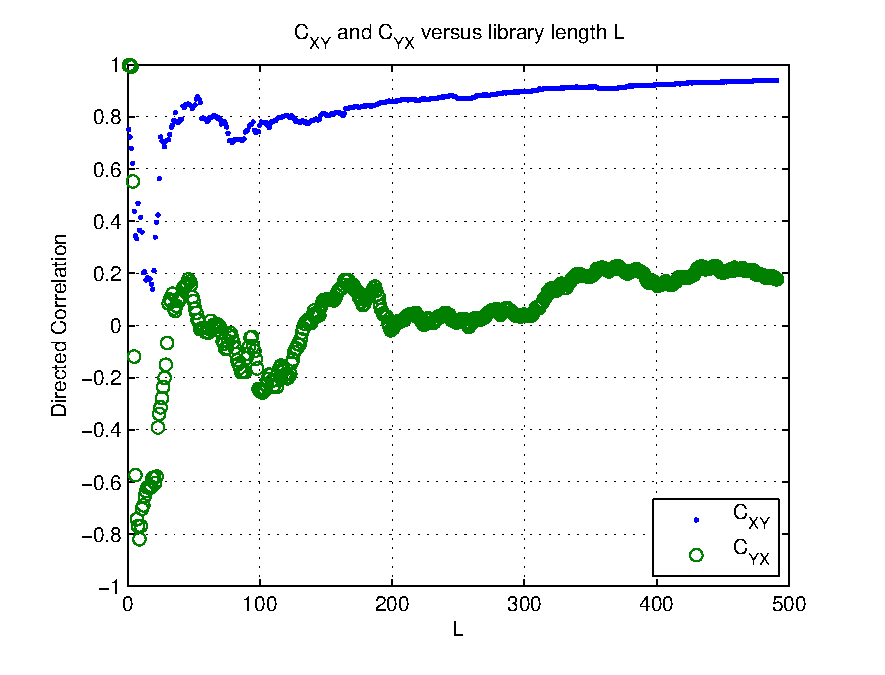
\includegraphics[scale=1]{CxyCyxVL.eps}
\caption{$\left(r_x,r_y,\beta_{xy},\beta_{yx},X(t_0),Y(t_0)\right) = \left(3.8,3.5,0.01,0.2,0.4,0.2\right)$ with $\tau=1$ and $E=2$.}
\end{figure}
Both directed correlations appear to converge to some nominal value and $C_{YX}<C_{XY}$ over most of the range (as expected).  But, notice that the small library length behaviour does not appear to follow expectations (i.e.\ $C_{YX}>C_{XY}$ for small $L$).

If instead the library length is fixed and the embedding dimension is varied, then the behaviour of the directed correlation changes dramatically.  Figure \ref{fig:CxyCyxVE} shows $C_{XY}$ and $C_{YX}$ calculated using all of the parameter values from above (and with $L=100$) but with the embedding dimension $E$ ranging from 2 to 50. 
\begin{figure}[h!t]
\label{fig:CxyCyxVE}
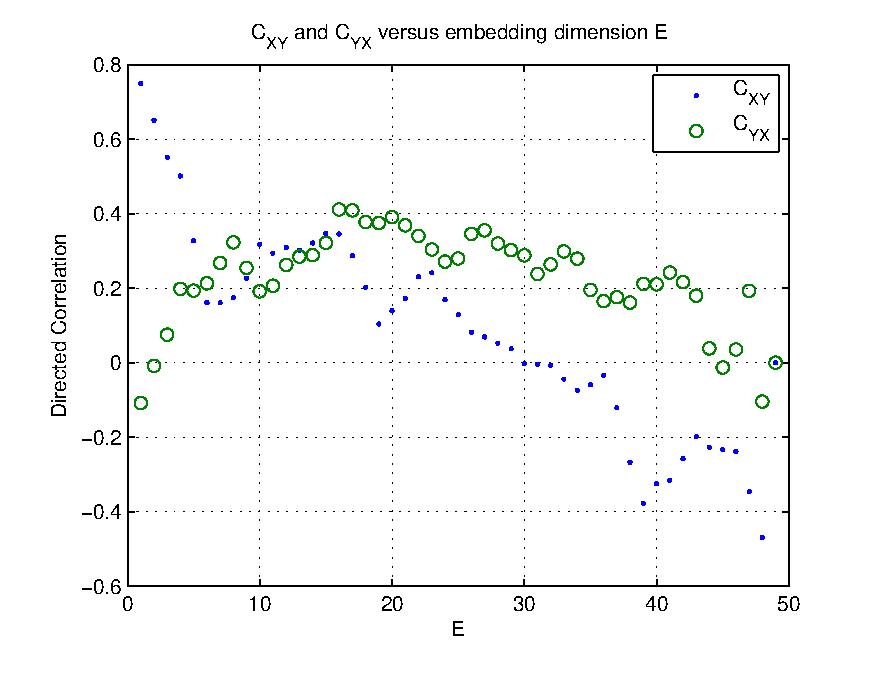
\includegraphics[scale=1]{CxyCyxVE.eps}
\caption{$\left(r_x,r_y,\beta_{xy},\beta_{yx},X(t_0),Y(t_0)\right) = \left(3.8,3.5,0.01,0.2,0.4,0.2\right)$ with $\tau=1$ and $L=100$.}
\end{figure}
There are points over the embedding range when $C_{YX}<C_{XY}$ but there are also points where $C_{YX}>C_{XY}$, which is difficult to interpret with the given parameter set.  The dependence on the embedding dimension is concerning because it implies that incorrect conclusions can be drawn about natural data sets (i.e.\ time series where the theoretical dynamics are not known) regarding which directed correlation is dominate (i.e.\ which time series is the dominate ``driver'').  Similar issues arise when plotting the directed correlation over a range for the time step $\tau$ from 1 to 25 (see Figure \ref{fig:CxyCyxVtau}).  
\begin{figure}[h!t]
\label{fig:CxyCyxVtau}
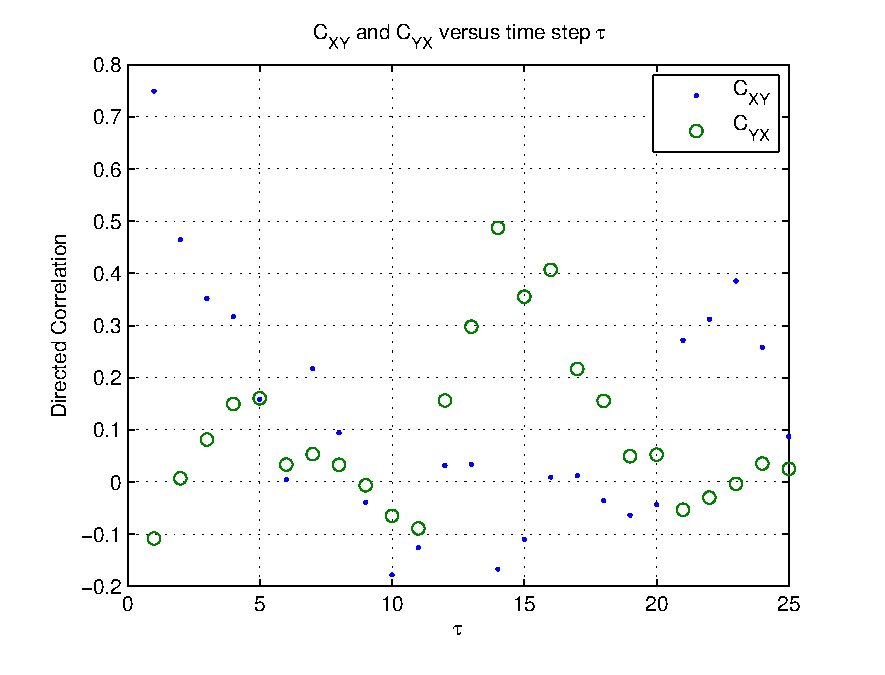
\includegraphics[scale=1]{CxyCyxVtau.eps}
\caption{$\left(r_x,r_y,\beta_{xy},\beta_{yx},X(t_0),Y(t_0)\right) = \left(3.8,3.5,0.01,0.2,0.4,0.2\right)$ with $E=2$ and $L=100$.}
\end{figure}

The directed correlation acts as expected for $L=100$, $E=2$, and $\tau=1$.  These values can be used (along with $r_x$ and $r_y$) to see how the directed correlation behaves over a range of $\beta_{yx}$ given $\beta_{xy}=0.5$.  Figure \ref{fig:CxyCyxVByx_raw} shows $C_{YX}$ and $C_{XY}$ plotted over the range $\beta_{yx}\in[0.01,1.0]$ (with $\beta_{xy}=0.5$), and Figure \ref{fig:CxyCyxVByx_diff} shows the difference $\Delta = (C_{XY}-C_{YX})$ over the same range.
\begin{figure}[h!t]
\label{fig:CxyCyxVByx_raw}
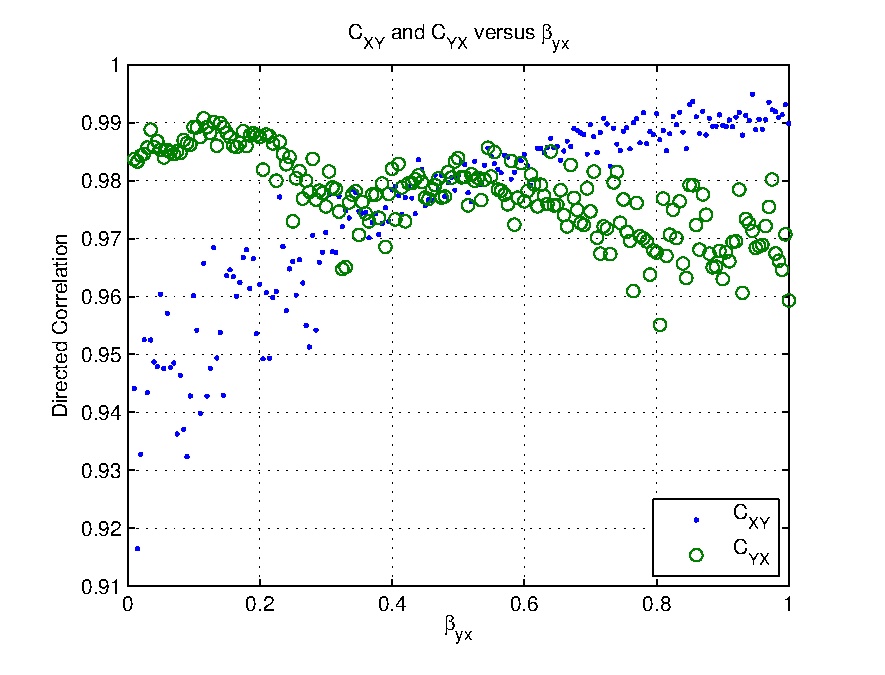
\includegraphics[scale=1]{CxyCyxVByx_raw.eps}
\caption{$\left(r_x,r_y,\beta_{xy},X(t_0),Y(t_0)\right) = \left(3.8,3.5,0.5,0.4,0.2\right)$ with $\left(E,L,\tau\right)=\left(2,500,1\right)$.}
\end{figure}
\begin{figure}[h!t]
\label{fig:CxyCyxVByx_diff}
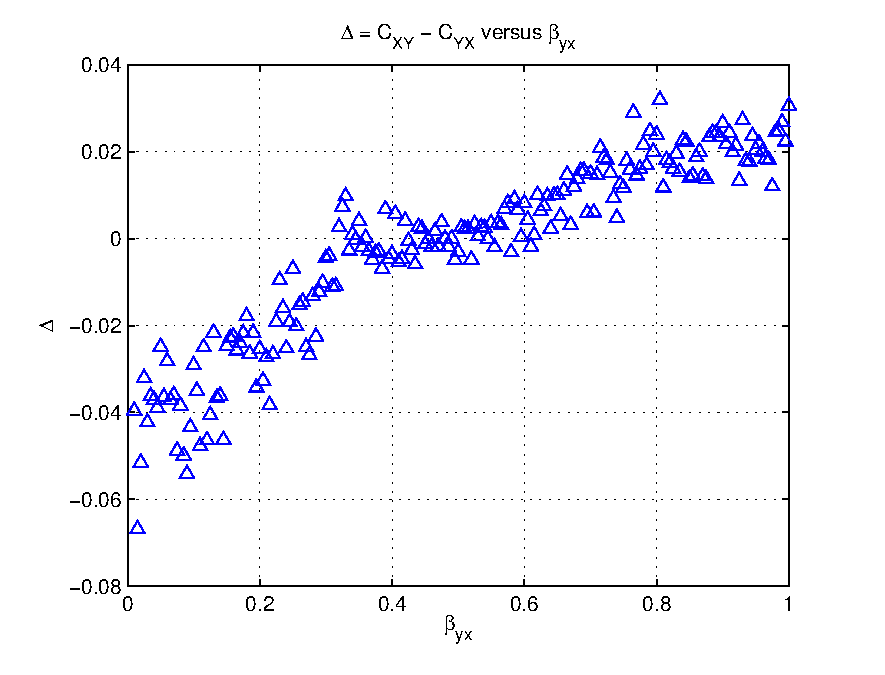
\includegraphics[scale=1]{CxyCyxVByx_diff.eps}
\caption{$\left(r_x,r_y,\beta_{xy},X(t_0),Y(t_0)\right) = \left(3.8,3.5,0.5,0.4,0.2\right)$ with $\left(E,L,\tau\right)=\left(2,500,1\right)$.}
\end{figure}
Notice that $\Delta$ is an increasing function of $\beta_{yx}$ that crosses zero around $\beta_{yx}=0.5$, as expected given the discussion of the CCM algorithm in the beginning sections.  Figure \ref{fig:CxyCyxVByxBxy_diff} is a plot of $\Delta$ of ranges for both coupling constants, i.e.\ $\beta_{xy}\in[0.01,1.0]$ and $\beta_{yx}\in[0.01,1.0]$.
\begin{figure}[h!t]
\label{fig:CxyCyxVByxBxy_diff}
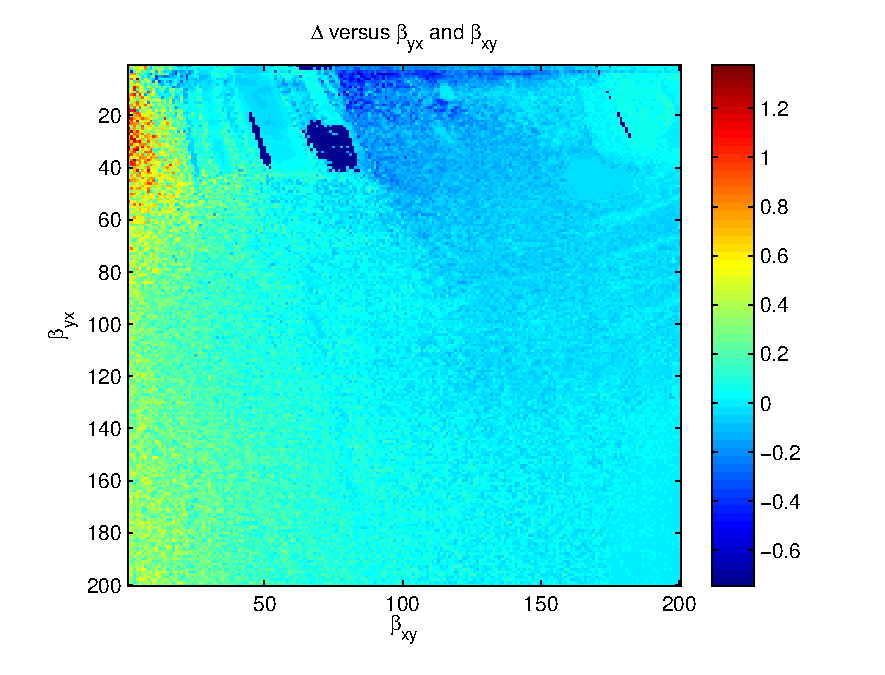
\includegraphics[scale=1]{CxyCyxVByxBxy_diff.eps}
\caption{$\left(r_x,r_y,X(t_0),Y(t_0)\right) = \left(3.8,3.5,0.2,0.4,0.2\right)$ with $\left(E,L,\tau\right)=\left(2,100,1\right)$.}
\end{figure}
Following the intuitive expectation, $\beta_{xy}>\beta_{yx}\Rightarrow \Delta<0$ and $\beta_{xy}<\beta_{yx}\Rightarrow \Delta>0$.

Notice,$\Delta$ is not symmetric about zero for the pair $(\beta_{xy},\beta_{yx})$; i.e.\
$$
\left(\beta_{xy},\beta_{yx}\right) = \left(0.5,0.01\right) \Rightarrow \Delta \approx -0.27\;\;,
$$
but
$$
\left(\beta_{xy},\beta_{yx}\right) = \left(0.01,0.5\right) \Rightarrow \Delta \approx 0.42
$$
which is positive but not 0.27.  The difference $\Delta$ is symmetric about zero given the entire parameter set for each time series, i.e.\
$$
\left(r_x,r_y,\beta_{xy},\beta_{yx},X(t_0),Y(t_0)\right) = \left(3.8,3.5,0.5,0.01,0.4,0.2\right) \Rightarrow \Delta \approx -0.27
$$
and
$$
\left(r_x,r_y,\beta_{xy},\beta_{yx},X(t_0),Y(t_0)\right) = \left(3.5,3.8,0.01,0.5,0.2,0.4\right) \Rightarrow \Delta \approx 0.27\;\;.
$$

Given the results of this section, the CCM algorithm does provide a kind of coarse grained quantification of the idea of ``driving'' between two time series.  More specifically, the sign of $\Delta$ provides information about the relative strength of dependencies between two time series.
\section{Applying CCM to Known Dynamics}
The results shown above for the example presented by Sugihara appear to imply the following:
\begin{enumerate}
\item The CCM method is not robust with respect to the embedding dimension (i.e.\ $E$) or lag time step (i.e.\ $\tau$).
\item The CCM method can lead to results that agree with intuition for the presented example. 
\end{enumerate}
These points will be explored by applying the CCM to two very different sets of dynamics.  The first will explore a driven system by comparing the directed correlations calculated between the voltage and current time series of an RL circuit, and the second will explore the directed correlations found in the Lorenz system, which is known to be chaotic.

\subsection{RL Circuit}
An RL circuit is described as
$$
\dot{I} = \frac{V}{L} - \frac{R}{L} I\;\;,
$$
where $I$ is the current, $V$ is the voltage, $R$ is the resistance, and $L$ is the inductance.  The driving time series will be the voltage $V$ and the response times series will be the current $I$.  The resistance and inductance will be considered fixed.

Consider an RL circuit with $(R,L) = (0.5,10)$.  If the voltage times series $V$ consists of two triangular pulses separated by constant spans of $V=0$, then the current times series $I$ will likewise has two maximums as seen in Figure \ref{fig:RL_trigsignals}.
\begin{figure}[h!t]
\label{fig:RL_trigsignals}
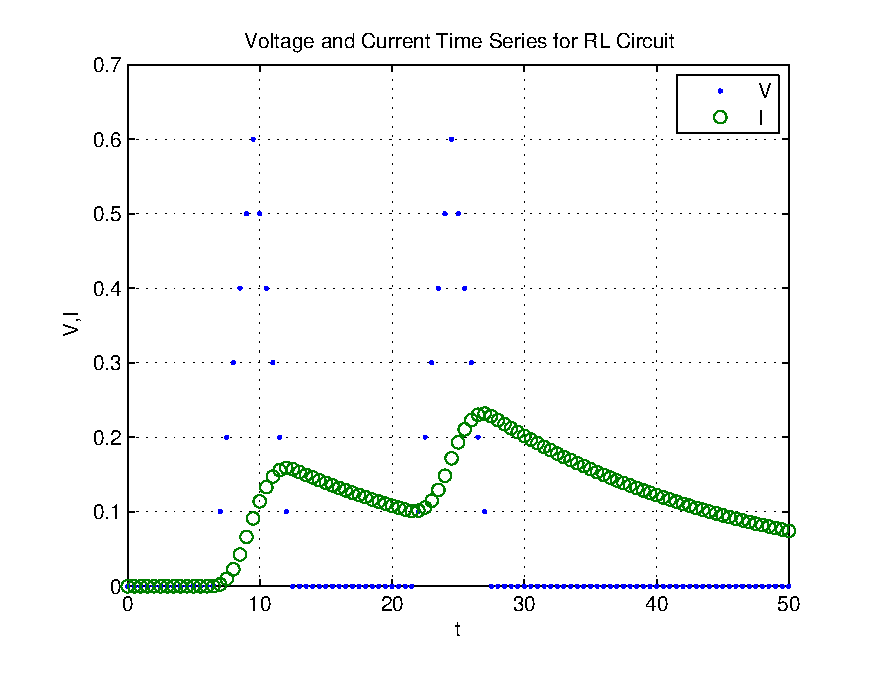
\includegraphics[scale=1]{RL_trigsignals.eps}
\caption{$(R,L) = (0.5,10)$}
\end{figure}
The directed correlations $C_{VI}$ and $C_{IV}$ can be plotted as a function of the embedding dimension $E$ to show that $C_{VI}>C_{IV}$ for $E=2,3,\ldots,10$.  This plot is Figure \ref{fig:RL_trigsignalsCCM}.
\begin{figure}[h!t]
\label{fig:RL_trigsignalsCCM}
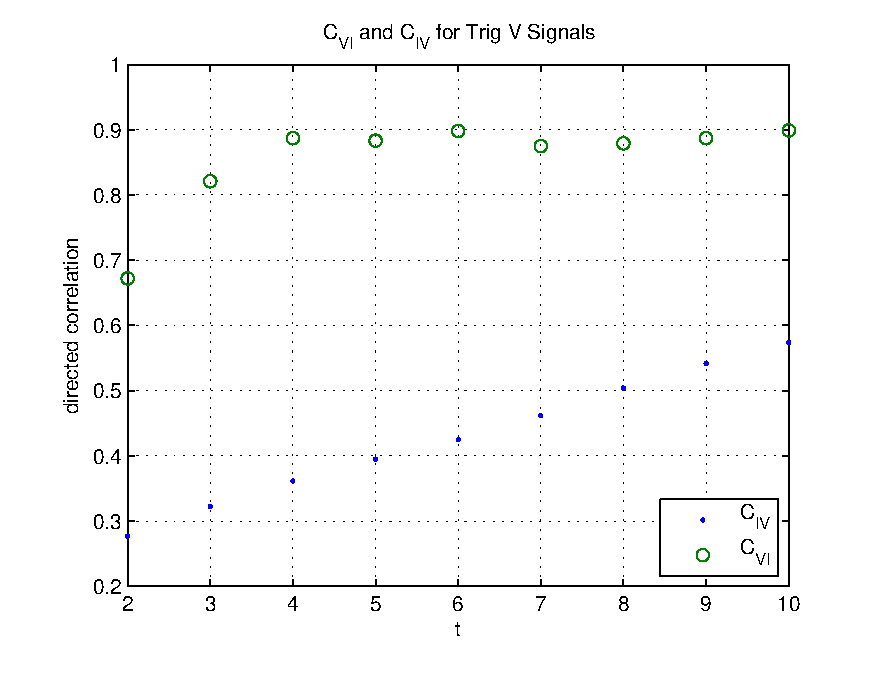
\includegraphics[scale=1]{RL_trigsignalsCCM.eps}
\caption{$(R,L) = (0.5,10)$ with $\left(E,L,\tau\right)=\left(2,100,1\right)$}
\end{figure}
This result (i.e.\ that the system is directionally correlated from $V$ to $I$) is expected because $V\Rightarrow I$ (i.e.\ the voltage drives the current).

Consider the case when $V$ is a discrete sine function; see Figure \ref{fig:RL_sinsignals} for a plot of the $V$ and $I$ times series.
\begin{figure}[h!t]
\label{fig:RL_sinsignals}
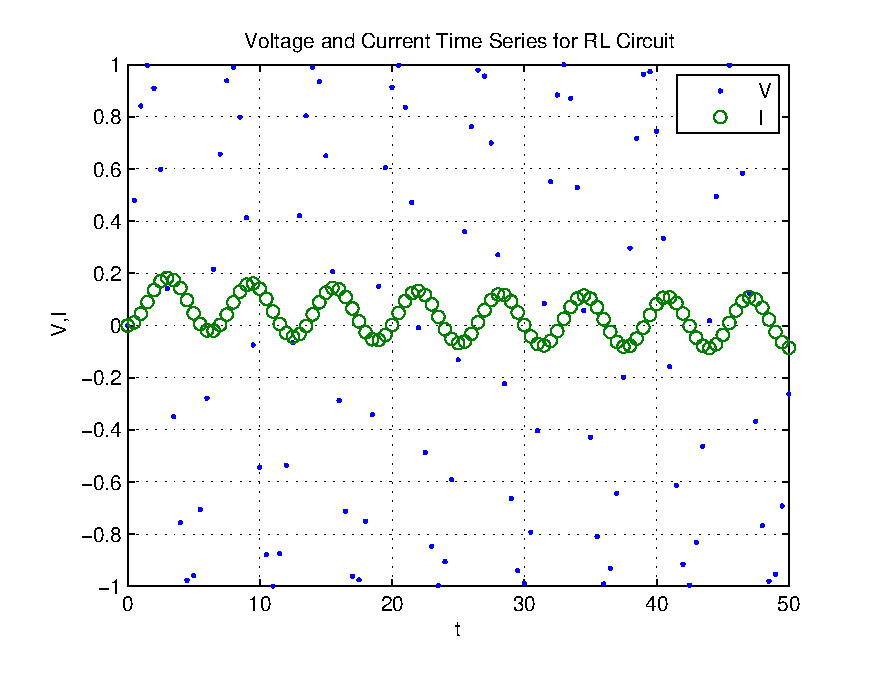
\includegraphics[scale=1]{RL_sinsignals.eps}
\caption{$(R,L) = (0.5,10)$}
\end{figure}
The values of $C_{VI}$ and $C_{IV}$ are different than they were in the example of the previous paragraph but the general relationship is the same, i.e.\ $C_{VI}>C_{IV}$ for $E=2,3,\ldots,10$.  See Figure \ref{fig:RL_sinsignalsCCM}.
\begin{figure}[h!t]
\label{fig:RL_sinsignalsCCM}
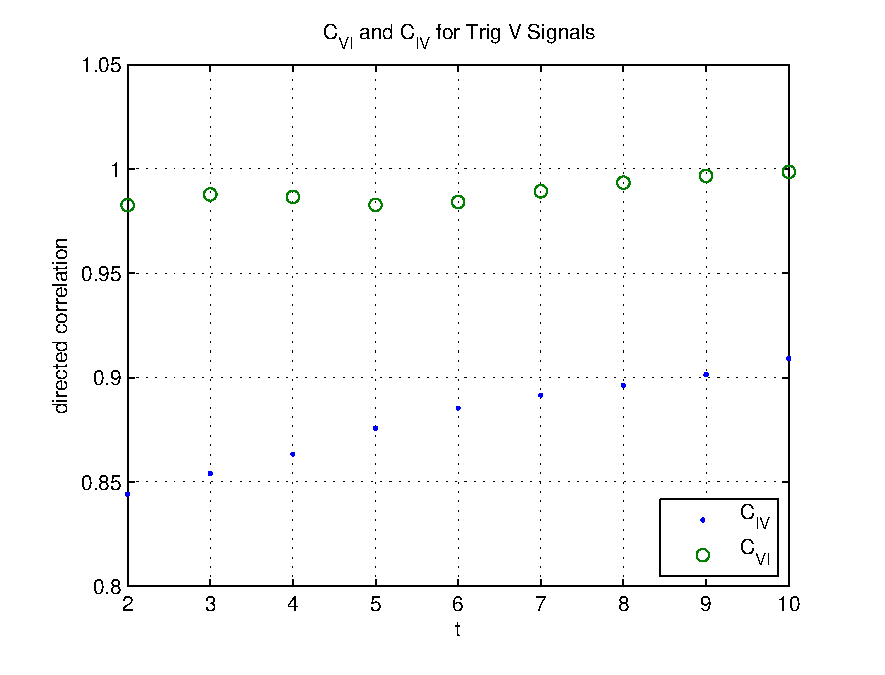
\includegraphics[scale=1]{RL_sinsignalsCCM.eps}
\caption{$(R,L) = (0.5,10)$ with $\left(E,L,\tau\right)=\left(2,100,1\right)$}
\end{figure}

The ``non-robust'' features of the directed correlations (with respect to $E$) can be recovered for the RL circuit by setting each point of $V$ to be a random value.  While such a voltage time series may be defined as ``unphysical'', it will illustrate the same $E$-dependent behavior of the directed correlations that was seen with the Sugihara example.  Consider the $V$ and $I$ times series of Figure \ref{fig:RL_randsignals}, where $V$ is a set of pseudo-random numbers generated with Matlab.
\begin{figure}[h!t]
\label{fig:RL_randsignals.eps}
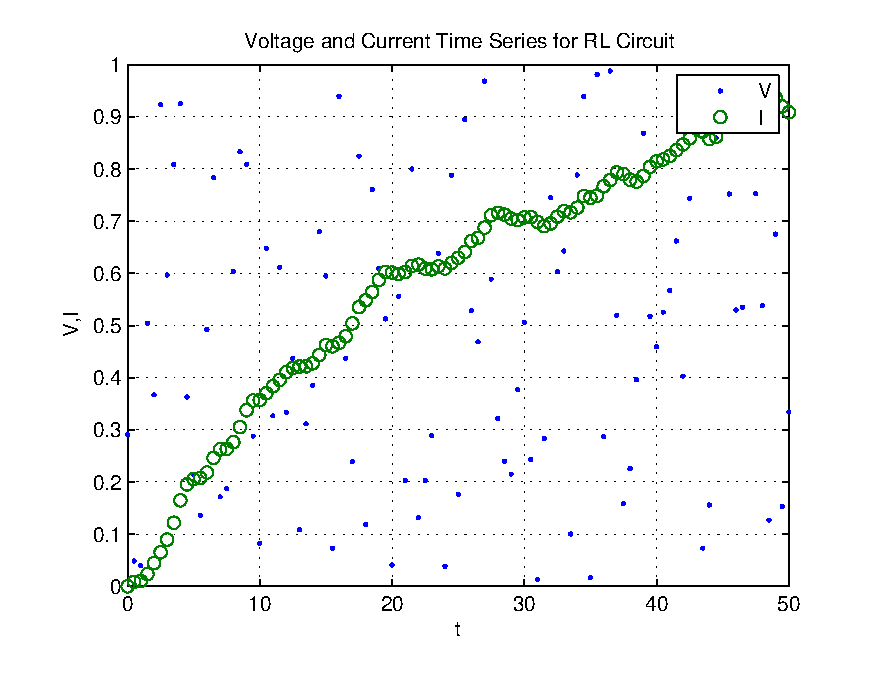
\includegraphics[scale=1]{RL_randsignals.eps}
\caption{$(R,L) = (0.5,10)$}
\end{figure}
The plot of $C_{VI}$ and $C_{IV}$ for $E=2,3,\ldots,10$ (see Figure \ref{fig:RL_randsignalsCCM})
\begin{figure}[h!t]
\label{fig:RL_randsignalsCCM}
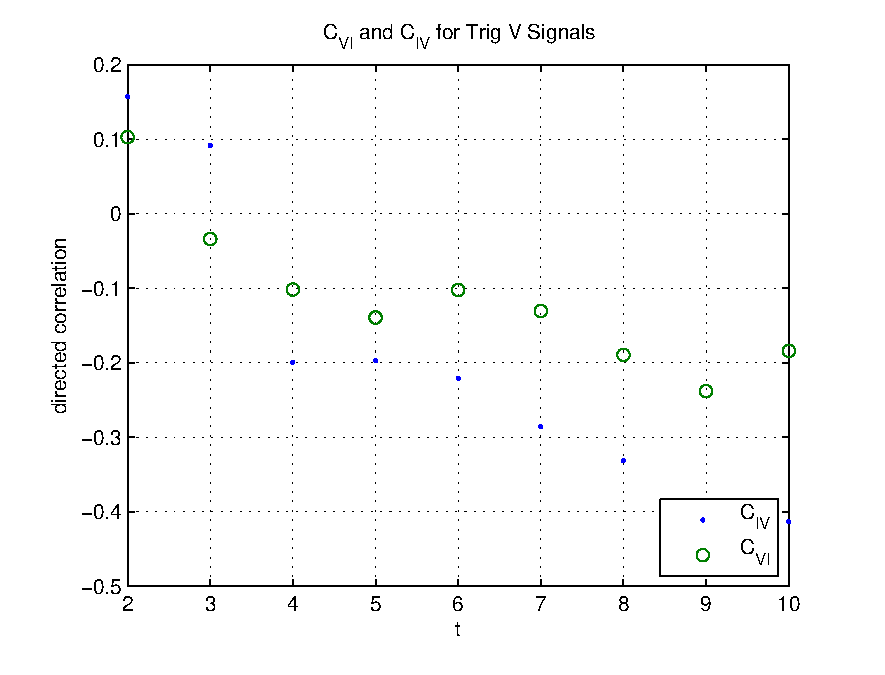
\includegraphics[scale=1]{RL_randsignalsCCM.eps}
\caption{$(R,L) = (0.5,10)$ with $\left(E,L,\tau\right)=\left(2,100,1\right)$}
\end{figure}
shows that $C_{VI}>C_{IV}$ if $E>= 4$ but $C_{VI}<C_{IV}$ if $E<4$ 

These results seem to imply that the robustness of the CCM method may be related to the autocorrelation of the ``driving'' time series.  This idea will be explored after the next section.

\subsection{Lorenz System}
Consider the following system of equations:
\begin{eqnarray*}
\dot{x} &=& \sigma\left(y-x\right)\\
\dot{y} &=& \rho x-y-xz\\
\dot{z} &=& xy - \beta z
\end{eqnarray*}
If $(\sigma,\beta,\rho)=(10,8/3,28)$, then the system's directed correlations are as follows:
\begin{eqnarray*}
C_{xy} &\approx & 0.91\\
C_{yx} &\approx & 0.94\\
C_{xz} &\approx & 0.11\\
C_{zx} &\approx & 0.88\\
C_{yz} &\approx & 0.08\\
C_{zy} &\approx & 0.45
\end{eqnarray*}
where $x(t)$, $y(t)$, and $z(t)$ are defined by the dynamical system at the beginning of this section.  These results seem to imply $z\Rightarrow x$ and $z\Rightarrow y$ with no conclusion for the relationship between $x$ and $y$.  These results seem confusing.  In particular, it seems to make sense that $z$ could be a stronger driver of $y$ than $y$ is of $z$ (i.e.\ $z\Rightarrow y$) but the implication that $z$ is a stronger driver of $x$ than $x$ is of $z$ (i.e.\ $z\Rightarrow x$) is more difficult to interpret given that $z$ only affects $x$ through $y$.


If $(\sigma,\beta,\rho)=(0.01,8/3,28)$, then the system's directed correlations are as follows:
\begin{eqnarray*}
C_{xy} &\approx & 0.79\\
C_{yx} &\approx & -0.12\\
C_{xz} &\approx & 0.90\\
C_{zx} &\approx & -0.74\\
C_{yz} &\approx & 0.47\\
C_{zy} &\approx & 0.71
\end{eqnarray*}
which implies $x\Rightarrow y$, $z\Rightarrow y$, and $x\Rightarrow z$.  Both $x\Rightarrow y$ and $x\Rightarrow z$ seems to make intuative sense given the smaller $\sigma$ in this example versus the previous example, and $z\Rightarrow y$ is consistent with the previous example which, again, makes sense because neither $\rho$ nor $\beta$ was changed.

If $(\sigma,\beta,\rho)=(10,0.01,28)$, then the system's directed correlations are as follows:
\begin{eqnarray*}
C_{xy} &\approx & -1\\
C_{yx} &\approx & 1\\
C_{xz} &\approx & 0.02\\
C_{zx} &\approx & 0.30\\
C_{yz} &\approx & 0.01\\
C_{zy} &\approx & 0.40
\end{eqnarray*}









\end{document}